% !TEX root = ../thesis-example.tex
%
\chapter{Introduction}
\label{chap:intro}

\begin{chapquote}{Antoine de Saint-Exupéry, \textsc{The Little Prince}}
Language is the source of misunderstandings.
\end{chapquote}

In this chapter, we present the motivation of this thesis, as well as related work on crowdsourcing ground truth for natural language processing. We introduce the CrowdTruth methodology for crowdsourcing ground truth while preserving inter-annotator disagreement. CrowdTruth is based on the idea that disagreement is not noise, but an important signal that can be used to capture ambiguity in the annotation data. We define the main research goal of how to interpret disagreement in crowdsourcing ground truth for natural language processing, along with four research questions that address this goal. Finally, we outline the main contributions of this thesis.

This chapter is based on the paper titled \textit{Crowdsourcing Disagreement for Collecting Semantic Annotation} in the European Semantic Web Conference~\cite{dumitrache2015crowdsourcing}.


\section{Motivation}

As knowledge available on the Web expands, natural language processing methods have become invaluable for facilitating data navigation. Tasks such as knowledge base completion and disambiguation are solved with machine learning models for natural language processing that require a lot of data. Human-annotated gold standard, or ground truth, is used for training, testing, and evaluation of these machine learning components. The traditional approach to gathering this data is to employ domain experts to perform annotation tasks.

However, such an annotation process can be both expensive, and time consuming~\cite{aroyo2012harnessing}, due to the costs of working with domain experts. Furthermore, experts might prove difficult to find for broad, open domains (e.g. the annotation of news articles). This presents a challenge for extending natural language processing methods into new domains. Human annotation is needed to solve this problem, but the process of gathering this data is not scalable at the level of the large datasets currently available on the Web. Efficiently integrating human knowledge with automated methods is necessary for tackling this issue. 

In recent years, crowdsourcing has become a viable alternative to using domain expert annotators, as it is both cheaper and more easily scalable~\cite{Sabou:2012:CRO:2362456.2362479}. This has been facilitated by platforms such as Amazon Mechanical Turk\footnote{\url{https://www.mturk.com/}} and Figure Eight\footnote{\url{https://www.figure-eight.com/}} (formerly known as Crowdflower) that offer readily available crowds of workers. The main challenge posed by crowdsourcing is how to tune the annotation tasks (e.g. in terms of worker selection, task question and template) in order to get the best quality of data~\cite{difallah2012mechanical}. The quality of the annotated data can have a big impact on the performance of machine learning models that learn from it -- so much so that Amazon has started offering a service\footnote{\url{https://aws.amazon.com/sagemaker/groundtruth/}} that optimizes the collection of human-labeled ground truth.

But what makes annotations high quality is still a matter of discussion. When collecting multiple annotations for the same task, it is likely that inter-worker disagreement will be present. In typical annotation setups it is assumed that one correct answer exists for every question, and that disagreement must be eliminated from the corpus. This traditional approach to gathering annotation, based on restrictive annotation guidelines, can often results in over-generalized observations, as well as a loss of ambiguity inherent to language~\cite{aroyo2012harnessing}, thus becoming unsuitable for use in training natural language processing systems. %Crowdsourcing allows for collecting enough annotations per task in order to represent the diversity inherent in language. By employing a large crowd to collect annotations, it becomes possible to observe inter-annotator disagreement.

The \textbf{CrowdTruth}\footnote{\url{http://crowdtruth.org}} methodology~\cite{aroyo2015truth,aroyo2013crowd,inel2013} has been proposed to perform crowdsourcing while preserving inter-annotator disagreement. CrowdTruth is based on the idea~\cite{aroyo2015truth} that disagreement is not noise, but an important signal that can be used to capture ambiguity in the annotated data. It considers the crowdsourcing system as a triangle~\cite{aroyo2014threesides} with three components that are inter-connected: workers, input data, and annotations. CrowdTruth captures inter-annotator disagreement and uses it to calculate a set of quality metrics\footnote{\url{https://github.com/CrowdTruth/CrowdTruth-core}} (Appendix~\ref{app:ct2.0}) for the three crowdsourcing components, by modeling the way that the components interact with each other -- e.g. in an ambiguous sentence, we expect to have more disagreement between workers, therefore workers on those sentences should not be considered less trustworthy. Previous research in crowdsourcing medical relation extraction~\cite{aroyo2013crowd,aroyo2013measuring} has shown that disagreement can be an informative, useful property, and its analysis can result in reduced time, lower cost, better scalability, and better quality human-annotated data.

This thesis explores how the CrowdTruth methodology can be used to collect ground truth data for the training and evaluation of natural language processing models. We present work done across several tasks (relation extraction, semantic frame disambiguation) and domains (medical, open), showing the role of inter-annotator disagreement beyond simply identifying low quality workers. We argue that disagreement does not need to be eliminated from ground truth data in order to preserve data quality. Furthermore, we show that disagreement is a valuable quality to preserve in ground truth data, that can be effectively used in the training and evaluation of natural language processing models. This is because inter-annotator disagreement is a powerful signal for the ambiguity that is inherent in natural language. Our goal is to break the constraints of the typical methodology for collecting ground truth, and prove that disagreement is a necessary characteristic of annotated data that, when interpreted correctly, can improve the performance of natural language processing models, and make evaluations more attuned to the noise in real-world data.


\section{Related Work}
\label{sec:intro-rel-work}

Crowdsourcing is a widely used method to collect natural language processing ground truth~\cite{Sabou:2012:CRO:2362456.2362479}. In this section, we explore background work on four important crowdsourcing issues: (1) how to establish crowd data quality, (2) how to aggregate multiple crowd annotations, (3) how natural language processing models use crowd data in training and evaluation, (4) and what the relation is between inter-worker disagreement and natural language ambiguity. These issues make up the backbone and the main topics that will be discussed in this thesis. The related work on these issues is composed of papers published in a wide variety of venues, across three main fields of artificial intelligence:   

\begin{itemize}
    \item \textit{human computation}, where the main venues are the Conference on Human Computation and Crowdsourcing (HCOMP), the Journal of Human Computation, the ACM Transactions on Interactive Intelligent Systems (TiiS) journal, and the Conference on Human Factors in Computing Systems (CHI);
    
    \item \textit{natural language processing}, and \textit{machine learning} more generally, where the main venues are the Annual Meeting of the Association for Computational Linguistics (ACL), the Conference on Empirical Methods in Natural Language Processing (EMNLP), the Annual Conference of the North American Chapter of the Association for Computational Linguistics (NAACL), and the Conference on Neural Information Processing Systems (NeurIPS);
    
    \item \textit{semantic web}, where the main venues are the International Semantic Web Conference (ISWC), the Extended Semantic Web Conference (ESWC), and the Semantic Web Journal.
\end{itemize}


\subsection{Crowd Data Quality}

Determining the quality of crowdsourced data collected from non-experts has been the subject of study since the work of \citet{Snow2008}, who have shown that the crowd can produce annotations with expert-level quality for a variety of natural language processing tasks: affect  recognition, word similarity, recognizing textual entailment, event temporal ordering, and word sense disambiguation. Despite these promising results, collecting high quality crowdsourced data is still a challenge, due primarily to the difficulty of identifying and preventing spam behavior of workers~\cite{difallah2012mechanical,demartini2012zencrowd}. This is especially the case when applying non-expert crowdsourcing to domains that are typically thought to require expertise on the part of the annotators~\cite{callison2010creating}.

The medical domain is particularly difficult, with even expert annotators sometimes producing low-quality data~\cite{Marcheggiani:2017:ELT:3139489.3106235}. Nevertheless, there exists some research that successfully employed non-expert crowdsourcing to collect annotations in the medical domain. \citet{mortensen2013crowdsourcing} use crowdsourcing to verify relation hierarchies in biomedical ontologies. On 14 relations from the SNOMED CT CORE Problem List Subset, the authors report the crowd's accuracy at 85\% for identifying whether the relations were correct or not. \citet{burger2012validating} used crowdsourcing to extract the gene-mutation relations in Medical Literature Analysis and Retrieval System Online (MEDLINE) abstracts. Focusing on a very specific gene-mutation domain, the authors report a weighted accuracy of 82\% over a corpus of 250 MEDLINE abstracts. \citet{li2015exposing} performed a study exposing ambiguities in a gold standard for drug-disease relations with crowdsourcing. They found that, over a corpus of 60 sentences, levels  of  crowd agreement varied in a similar manner to the levels of agreement  among  the  original  expert  annotators. \citet{zhai2013web} describe a method for crowdsourcing a ground truth for medical named entity recognition and entity linking. In a dataset of over 1,000 clinical trials, the authors show no statistically significant difference between the crowd and expert-generated gold standard for the task of extracting medications and their attributes.

Other difficult annotation tasks involve linguistics knowledge. For instance, frame disambiguation requires an understanding of the frame semantics theory~\cite{baker1998berkeley}, which can be difficult to explain to a crowd of non-experts. While \citet{Hong:2011:GCR:2018966.2018970} showed a high accuracy when comparing the crowd to experts for the task of frame disambiguation by simply calculating the majority vote, \citet{chang2015scaling} claim that a more complex multi-step annotation process is required in order to correct misunderstandings of the frame definition by the crowd.

In all of these experiments, disagreement between annotators is seen as undesirable and a sign of low quality data. In contrast, \citet{jurgens2013embracing} argues that ambiguity is an inherent feature of frame/word sense disambiguation, and that crowdsourcing can be used to capture it, by asking annotators to rate ambiguous examples on a Likert scale. Similarly, this thesis proposes that ambiguity is a useful property of natural language, but instead of asking workers directly to rate ambiguity, we study it through measuring inter-annotator disagreement. This presents an interesting challenge, as disagreement is usually removed from annotated datasets in order to improve their quality. Our goal in this work is to show that crowdsourced ground truth can still have quality comparable to that of domain experts, while still preserving the signals of worker disagreement.


\subsection{Crowdsourcing Aggregation Methods}
\label{sec:rel-work-agg}

The most common way to aggregate crowd annotations is majority voting, where the label for an example is picked based on whether or not the majority of crowd workers agree that it exists. Inter-annotator agreement in crowdsourcing is usually employed as a method to determine the quality of the annotations. Typically, disagreement is considered an undesirable feature of the annotations -- a byproduct either of low quality of the workers, or of an unclear annotation task. There are several metrics to capture inter-annotator agreement, most popular being Cohen's $\kappa$~\cite{cohen1960kappa} and Krippendorff's $\alpha$~\cite{klaus2013content}. \citet{artstein2008inter} compared several of these metrics, finding that the choice of metric is not as important as it is to increase the number of annotators, in order to reduce the prevalence of personal bias.

In recent years, there is also a growing body of research on alternative crowdsourcing aggregation metrics. There is a particular focus on modeling the reliability of crowd workers, by identifying spam workers~\cite{Bozzon:2013,Kittur2008,Ipeirotis:2010}, and analyzing workers' performance for quality control and optimization of the crowdsourcing processes~\cite{Singer:2013}. \citet{NIPS2009_3644} and \citet{welinder2010multidimensional} have used a latent variable model for task difficulty, as well as latent variables to measure the skill of each annotator, to optimize crowdsourcing for image labels. \citet{werling2015job} use on-the-job learning with Bayesian decision theory to assign the most appropriate workers for each task, for both text and image annotation. \citet{prelec2017solution} show that the surprisingly popular crowd choice (i.e. the answer that most workers thought would not be picked by other workers, even though it is correct) gave better results than the majority vote for a variety of tasks with unambiguous ground truths (state capitals, trivia questions and price of artworks). Finally, \citet{paun2018comparing} compare majority vote with 6 different Bayesian methods that aggregate crowd results while also modeling worker reliability and task item difficulty. The evaluation over a variety of task settings (binary and multiple choice, different levels of quality for the workers) shows 5 out of 6 of the Bayesian methods consistently outperform majority vote.

Our research is part of this current trend of investigating the limitations of majority vote as a crowdsourcing aggregation method. The novel approach of CrowdTruth is the modeling of ambiguity as a latent variable of the crowdsourcing system, that is present in inter-worker disagreement. Therefore, instead of discarding it, the CrowdTruth approach preserves disagreement and uses it to identify ambiguous data points. In this thesis, we will show that the CrowdTruth method to aggregate crowdsourcing annotations is applicable to a variety of annotation tasks, where simply using majority vote would result in the loss of important information regarding the ambiguity in the data.


\subsection{Natural Language Processing with the Crowd}
% add frames

Due to being both cheaper and more readily available than domain experts, crowdsourcing is used to collect training data for a variety of natural language processing tasks, across several domains: medical entity extraction~\cite{zhai2013web,Finin2010,van2012eu}, medical relation extraction~\cite{kilicoglu2011constructing,van2012eu}, open-domain relation extraction~\cite{kondreddi2014combining}, clustering and disambiguation~\cite{Lee2013}, ontology evaluation~\cite{noy2013mechanical}, web resource classification~\cite{castano2016human} and taxonomy creation~\cite{bragg2013crowdsourcing}. \citet{Snow2008} have shown that aggregating the answers of an increasing number of unskilled crowd workers with majority vote can lead to high quality natural language processing training data.

In this thesis, we focus on the training of one natural language processing task -- relation extraction from sentences. This task usually requires large amounts of training data, meaning that completely crowdsourcing the ground truth is cost-prohibitive. However, active and semi-supervised methods can be used to scale-up the signal in labeled data to unlabeled examples. \citet{angeli2014combining} used an active learning approach to identify candidate sentences for crowd labeling that will most impact the performance of their relation extraction model. \citet{levy2017zero} have shown that a small crowdsourced dataset of questions about relations can be exploited to perform zero-shot learning. \citet{pershina2014infusion} used a small dataset of hand-labeled data to generate relation-specific guidelines that are used as additional features in the relation extraction.

The approach in these works is to restrict disagreement between annotators by using either of the following methods: restricting annotator guidelines, picking one answer that reflects some consensus usually through majority voting, or using a small number of annotators. In this thesis, we explore the question of whether crowdsourced data that preserves disagreement can be used as ground truth for the task of relation classification in sentences. We investigate whether inter-annotator disagreement in particular is a useful signal that the relation classification model can learn from, and whether our crowdsourcing method can be scaled-up through a semi-supervised learning approach.


\subsection{Capturing Ambiguity}
\label{sec:rel-work-ambig}

Our work is part of a continuous effort in exploring the link between inter-annotator disagreement and ambiguity of the input data, as applied to a variety of tasks and domains.

In an experiment for crowdsourcing anaphora resolution, \citet{poesio2005reliability} found that inter-annotator disagreement is linked to ambiguity in the text, and that directly asking the annotators to identify the ambiguous annotations is not enough to identify all the implicitly ambiguous cases. In assessing the OAEI benchmark, \citet{cheatham2014conference} found that disagreement between annotators (both crowd and expert) is an indicator for inherent uncertainty in the domain knowledge, and that current benchmarks in ontology alignment and evaluation are not designed to model this uncertainty. \citet{plank-hovy-sogaard:2014:P14-2} found similar results for the task of crowdsourced part-of-speech tagging -- most inter-annotator disagreement was indicative of debatable cases in linguistic theory, rather than faulty annotation. \citet{Bayerl2011} also investigate the role of inter-annotator disagreement as a possible indicator of ambiguity inherent in natural language. \citet{Chang:2017:Revolt} found that ambiguous cases cannot simply be resolved by better annotation guidelines or through worker quality control. Across a series of textual annotation tasks, \citet{chang2016linguistic} found that the vast majority of annotators that disagree with the gold standard were correct in their assessment, either because the gold standard was faulty, or the task allowed for multiple correct answers. %\citet{lau2014measuring} propose a method for crowdsourcing ambiguity in the grammatical correctness of text by giving workers the possibility to pick various degrees of correctness, but inter-annotator disagreement is not discussed as a factor in measuring this ambiguity.

 Beyond text, studies in the annotation of music similarity~\cite{doi:10.1080/09298215.2016.1200631}, time series~\cite{schaekermann2016,schaekermann2018resolvable}, and medical images~\cite{cheplygina2018crowd} have shown that disagreement between annotators can be an indicator for interesting properties of the data, such as ambiguity and uncertainty.
 
 In most of these works, ambiguity is treated like a curious outlier, a property of the data that is unclear how it should be handled. We claim that ambiguity is an inherent part of natural language, and should be treated as such, by clearly defining it in ground truth corpora, and using it for training and evaluation of natural language processing models. %We achieve this through a comparative analysis that shows how ambiguity, as measured with disagreement-preserving CrowdTruth metrics, is present across several tasks and domains.


\section{Research Questions \& Contributions}

Based on the issues we identified in Section~\ref{sec:intro-rel-work}, the overall goal of this thesis is to \textit{investigate the role of inter-annotator disagreement in crowdsourcing ground truth for natural language processing}, as collected using CrowdTruth methodology and metrics. The main research goal is addressed by answering the following research questions:

\begin{itemize}
    \item \textbf{RQ1:} \textit{Does allowing disagreement in crowdsourcing ground truth yield the same quality as asking domain experts?}
    
    Chapter~\ref{chap:med-rel-ex} explores this question for the task of medical relation extraction. In the medical domain it is typically assumed that expert annotators are required to get the best quality ground truth. This work shows that, by capturing the inter-annotator disagreement with the CrowdTruth method, medical relation classifiers trained on crowd annotations perform the same as those trained on expert annotations. Furthermore, classifiers trained on crowd annotations perform better than those trained with automatically-labeled data. Using the crowd also reduces the cost (monetary and in time required to find annotators) for collecting the data. This chapter is based on the following publication:
    
    \begin{itemize}
        \item Dumitrache, Anca, Lora Aroyo, and Chris Welty. ``Crowdsourcing ground truth for medical relation extraction.'' \textit{ACM Transactions on Interactive Intelligent Systems (TiiS)} 8.2 (2018): 12.~\cite{DBLP:journals/corr/DumitracheAW17}
    \end{itemize}

    \item \textbf{RQ2:} \textit{How does allowing disagreement in diverse crowdsourcing tasks influence the quality of the data?}
    
    Chapter~\ref{chap:maj-vote} compares the quality of crowd data aggregated with CrowdTruth metrics and majority vote, a consensus - enforcing metric, over a diverse set of crowdsourcing tasks. We show that, by applying the CrowdTruth methodology, we collect richer data that allows us to reason about ambiguity of content. Furthermore, an increased number of crowd workers leads to growth and stabilization in the quality of annotations, going against the usual practice of employing a small number of annotators. This chapter is based on the following publication:
    
    \begin{itemize}
        \item Dumitrache, Anca, et al. ``Empirical methodology for crowdsourcing ground truth.'' \textit{Semantic Web Journal}. 2019 (in publication).~\cite{dumitracheempirical}
    \end{itemize}

    \item \textbf{RQ3:} \textit{Can we improve the performance of natural language processing models by using disagreement-aware ground truth data?}
    
    In Chapter~\ref{chap:od-rel-ex} we discuss how CrowdTruth data can be used to better models for relation classification for sentences. We build on work from Chapter~\ref{chap:med-rel-ex}, where we have shown that training models on on crowd annotations gives better results than training with data automatically-labeled with distant supervision~\cite{mintz2009distant}. However, crowd data is expensive to collect. Chapter~\ref{chap:od-rel-ex} describes how to correct a large corpus of training data for relation classification by using only a relatively small crowdsourced corpus, with two different methods: (1) by manually propagating the false positive and cross-relation signals identified with the help of the crowd, and (2) by adapting the semantic label propagation method~\cite{sterckx2016knowledge} to work with CrowdTruth data. This chapter is based on the following publications:
    
    \begin{itemize}
        \item Dumitrache, Anca, Lora Aroyo, and Chris Welty. ``False positive and cross-relation signals in distant supervision data.'' \textit{Proceedings of the Sixth Workshop on Automated Knowledge Base Construction (AKBC) at NIPS}. 2017.~\cite{dumitrache2017false}
        
        \item Dumitrache, Anca, Lora Aroyo, and Chris Welty. ``Crowdsourcing semantic label propagation in relation classification.'' \textit{Proceedings of the First Workshop on Fact Extraction and VERification (FEVER) at EMNLP}. 2018.~\cite{dumitrache2018crowdsourcing}
    \end{itemize}

    \item \textbf{RQ4:} \textit{Is inter-annotator disagreement an accurate indicator for ambiguity in natural language?}
    
    In Chapter~\ref{chap:frames}, we explore this question as applied to the task of disambiguating semantic frames (i.e. high-level concepts that represent the meanings of words). Similarly to Chapter~\ref{chap:med-rel-ex}, we show that the crowd achieves comparative quality with domain experts. A qualitative evaluation of cases when crowd and expert disagree shows that inter-annotator disagreement is an indicator of ambiguity in both frames and sentences. We demonstrate that the cases in which the crowd workers could not agree exhibit ambiguity, either in the sentence, frame, or the task itself, arguing that collapsing such cases to a single, discrete truth value (i.e. correct or incorrect) is inappropriate, creating arbitrary targets for machine learning. This chapter is based on the following publication:
    
    \begin{itemize}
        \item Dumitrache, Anca, Lora Aroyo, and Chris Welty. ``Capturing ambiguity in crowdsourcing frame disambiguation.'' \textit{Proceedings of the Sixth AAAI Conference on Human Computation and Crowdsourcing (HCOMP)}. 2018.~\cite{DBLP:conf/hcomp/DumitracheAW18}
        \item Dumitrache, Anca, Lora Aroyo, and Chris Welty. ``A crowdsourced frame disambiguation corpus with ambiguity.'' \textit{Proceedings of the Annual Conference of the North American Chapter of the Association for Computational Linguistics (NAACL-HLT).} 2019 (in publication).~\cite{dumitrache2019frames}
    \end{itemize}
\end{itemize}

In addition to addressing these research question, this thesis also contributes a collection of datasets, across different tasks and domains, that have been collected with crowdsourcing and processed with the CrowdTruth methodology for disagreement analysis to capture ambiguity:

\begin{enumerate}
    \item 3,984 English sentences for \textit{medical relation extraction}, centering on the $cause$ and $treat$ relations~\cite{anca_dumitrache_2016_50676};
    
    \item 4,100 sentences annotated with {\textit open domain relation extraction}, centering on 16 popular relations between $Person$, $Location$ and $Organization$ term types~\cite{crowdODrelexdata2016};
    
    \item 433 sentence-word pairs from the FrameNet corpus, and 5,000 sentence-word pairs from Wikipedia annotated with \textit{frame disambiguation}~\cite{anca_dumitrache_2018_1472345}.
\end{enumerate}


As another contribution, we have developed the CrowdTruth methodology as an open-source {\textit software package}.\footnote{\url{https://github.com/CrowdTruth/CrowdTruth-core}} Unlike other aggregation methods, our goal is to preserve dissenting annotations into a richer, continuous representation of truth. The disagreement is used to calculate quality scores for the crowd task input data, annotations and annotators. The complete definition of the CrowdTruth quality scores is given in Appendix~\ref{app:ct2.0}. The CrowdTruth software implements this methodology as a Python package, calculating the quality scores from raw data collected from crowdsourcing platforms. We offer support for a variety of crowdsourcing tasks, both closed and open-ended.  To facilitate the usage of our software, we provide a tutorial\footnote{\url{http://crowdtruth.org/tutorial/}} that discusses its application in a series of diverse use cases for collecting human annotation.





% The central characteristic of CrowdTruth is harnessing the diversity in human interpretation to capture the wide range of opinions and perspectives, and thus, provide more reliable and realistic real-world annotated data for training and evaluating machine learning components.

%another contribution of this thesis is a collection of ground truth datasets for the tasks of medical relation extraction~\cite{anca_dumitrache_2016_50676}, open domain relation extraction~\cite{crowdODrelexdata2016}, and semantic frame disambiguation~\cite{anca_dumitrache_2018_1472345}. These datasets have been collected with crowdsourcing and processed with the CrowdTruth methodology. The disagreement-aware metrics have allowed us to label the data with continuous truth labels for sentences, relations, semantic frames and workers, allowing us to capture the ambiguity inherent in these tasks.

% add appendix with all data sources & Github code

% \section{Crowdsourcing with CrowdTruth}

% To address the challenge of capturing an interpreting disagreement in crowdsourced annotations, we have proposed the \textbf{CrowdTruth methodology}~\cite{aroyo2012harnessing,aroyo2013crowd}. The goal of this methodology is to correct the myths of human annotation proposed by~\citet{aroyo2015truth}:

% \begin{itemize}

%     % Disagreement is a useful signal
%     % Multiple annotators are better
%     % Annotation guidelines should be short and to the point
%     % A continuous notion of truth

%     \item \textit{Myth \#1: Disagreement is bad -} This myth holds that, whenever inter-annotator disagreement occurs, it is the fault of the annotators. Therefore disagreement should be eliminated at all cost. In contrast, CrowdTruth proposes the idea that disagreement can also be caused by ambiguity in the annotation task. Specifically for the case of natural language, ambiguity is an inherent property of text. CrowdTruth proposes that capturing disagreement is a method to capture this ambiguity.
    
%     \item \textit{Myth \#2: One is enough -} Following from the previous myth, if inter-annotator disagreement can be an important indicator, then having a single worker perform the annotations means missing out on the signal the disagreement can send. CrowdTruth proposes using multiple workers for the same annotation task, in order to collect all possible disagreement that can occur.
    
%     \item \textit{Myth \#3: Experts are better -} While traditional annotation tasks ask a single domain expert to give their input, CrowdTruth proposes expanding this singular perspective with that of crowd workers. That is not to say that the experts are not necessary, or that the crowd is better suited at understanding an annotation task, just that often the perspective of the crowd is necessary in order to get a more accurate overview.
    
%     \item \textit{Myth \#4: One truth -} This myth holds that, for each annotation task, there is only one possible truth to how it should be done. Instead of forcing annotations into binary labels that are either positive or negative, CrowdTruth proposes that the truth exists on a scale, and is expressed with various degrees of clarity.
    
%     \item \textit{Myth \#5: All examples are equal -} If the truth value of a label is expressed on a scale, then it follows that there exists some variability in how clear a label is expressed in different examples. For instance, for the task of text labeling, some texts might express the desired label more clearly than others. The CrowdTruth methodology attempts to capture the degree of clarity of each example in the annotation task through the use of dedicated metrics, thus quantifying the fact that not all examples are equal in how well they express a label.
    
%     \item \textit{Myth \#6: Detailed guidelines help -} Typical annotation practice which provides detailed annotation guidelines to workers, which result in brittle overly-specific interpretations of the annotations. In contrast, the CrowdTruth methodology employs simple annotation guidelines that allow for disagreement over the interpretation of annotations.
    
% \end{itemize}

% The \textbf{CrowdTruth quality metrics}~\cite{aroyo2014threesides} are designed to capture the level of agreement associated with each component in the crowdsourcing system: workers, task annotations, and input media units. To address the myths of annotations discussed previously, the metrics measure quality on a scale -- e.g. instead of attributing binary labels to workers in order to determine whether or not they are spammers, we calculate a quality score that informs us the degree to which the worker is reliable. The main CrowdTuth quality metrics are:

% \begin{itemize}
%     \item \textit{Media Unit Quality Score (UQS)} -- the overall worker agreement over one media unit;
%     \item \textit{Worker Quality Score (WQS)} -- the overall agreement of one crowd worker with the other workers that annotated the same media units, calculated as a product of 2 other metrics:
%     \begin{itemize}
%         \item \textit{Worker-Worker Agreement (WWA)} -- the pairwise agreement between a given worker and all other workers, across all media units they annotated in common;
%         \item \textit{Worker-Media Unit Agreement (WUA)} -- the similarity between the annotations of a worker and the aggregated annotations of the rest of the workers;
%     \end{itemize}
%     \item \textit{Annotation Quality Score (AQS)} -- the agreement over an annotation in all media units that it appears;
%     \item \textit{Media Unit - Annotation Score (UAS)} -- the degree of clarity with which an annotation is expressed in a media unit.
% \end{itemize}

% In order to compute the CrowdTruth quality metrics, we need to formalize crowd annotations into a \textit{vector space representation}. For every input media unit, the annotations of each worker form a binary \textit{worker vector}, where the annotations selected are equal to `1', and the rest to `0'. The \textit{media unit vector} is the sum of all worker vectors for the given media unit. The first version of the CrowdTruth methodology~\cite{inel2014crowdtruth} calculates the metrics using cosine similarity over the vector representations of the crowd annotations.

% Version 2.0 of the CrowdTruth methodology~\cite{dumitrache2018crowdtruth} is explicitly modeled on the triangle of disagreement (Figure~\ref{fig:triangle_of_disagr}). Based on the triangle of reference \cite{knowlton1966definition}, it links together media units, workers, and annotations. The triangle model expresses how ambiguity in any of the corners disseminates and influences the other components of the triangle. The propagation of ambiguity in the triangle system is made explicit through making the quality metrics mutually dependent. For example, the quality of a worker is weighted by the quality of the media units the worker has annotated, and the quality of the annotations in the task -- this is because we expect an unclear sentence or an ambiguous annotation scheme would cause more disagreement between workers.

% \begin{figure}[!htb]
%  	\centering
%  		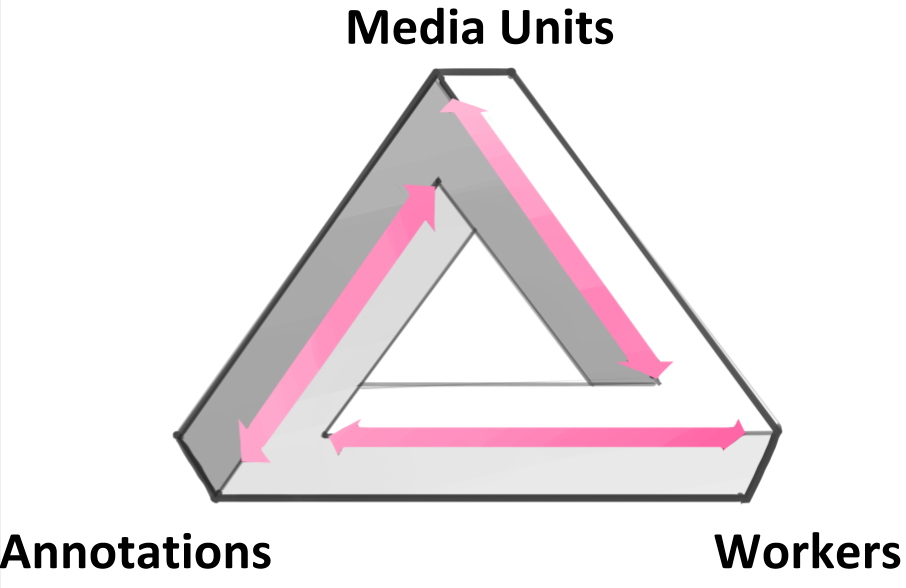
\includegraphics[width=0.5\linewidth]{img/triangle.png}
%  	\caption{Triangle of Disagreement}
%  	\label{fig:triangle_of_disagr}
%  \end{figure}

% in this thesis we apply CrowdTruth to a variety of NLP tasks and see what is the role of disagreement